\documentclass[12pt,a4paper]{article}

% ===== BASIC PACKAGES =====
\usepackage{fontspec}
\setmainfont{Times New Roman}

% ===== VIETNAMESE SUPPORT =====
\usepackage{polyglossia}
\setdefaultlanguage{vietnamese}
\setotherlanguage{english}

% ===== PAGE LAYOUT =====
\usepackage[a4paper,top=2.5cm,bottom=2.5cm,left=3cm,right=2.5cm]{geometry}
\usepackage{setspace}
\onehalfspacing

% ===== GRAPHICS AND TABLES =====
\usepackage{graphicx}
\usepackage{booktabs}
\usepackage{float}
\usepackage{caption}
\usepackage{longtable}

% ===== COLORS =====
\usepackage{xcolor}
\definecolor{hustred}{HTML}{ce1628}
\definecolor{hustblue}{HTML}{005a8c}

% ===== HYPERLINKS =====
\usepackage[colorlinks=true,linkcolor=hustblue,urlcolor=hustblue]{hyperref}

% ===== ENUMERATION =====
\usepackage{enumitem}

% ===== CODE LISTING =====
\usepackage{listings}
\lstset{
  basicstyle=\small\ttfamily,
  keywordstyle=\color{hustblue}\bfseries,
  stringstyle=\color{hustred},
  commentstyle=\color{gray}\itshape,
  numbers=left,
  numberstyle=\tiny\color{gray},
  numbersep=8pt,
  frame=single,
  breaklines=true,
  showstringspaces=false,
  tabsize=4,
  backgroundcolor=\color{gray!5},
  xleftmargin=1cm,
  framexleftmargin=1cm,
}

% ===== HEADER AND FOOTER =====
\usepackage{fancyhdr}
\setlength{\headheight}{14.5pt}
\pagestyle{fancy}
\fancyhf{}
\fancyhead[L]{\small\textcolor{hustred}{HUST - SoICT}}
\fancyhead[R]{\small\textcolor{hustred}{IT6130 - Lập trình và Ảo hóa cho IoT}}
\fancyfoot[C]{\thepage}
\renewcommand{\headrulewidth}{0.4pt}

% ===== SECTION FORMATTING =====
\usepackage{titlesec}
\titleformat{\section}{\Large\bfseries\color{hustred}}{\thesection.}{0.5em}{}
\titleformat{\subsection}{\large\bfseries\color{hustblue}}{\thesubsection.}{0.5em}{}
\titleformat{\subsubsection}{\normalsize\bfseries}{\thesubsubsection.}{0.5em}{}

% ===== GRAPHICS PATH =====
\graphicspath{{./}{../docs/images/}}

% ========================================
\begin{document}
\sloppy

% ===== TITLE PAGE =====
\begin{titlepage}
\thispagestyle{empty}
\begin{center}
    \normalsize{\textbf{ĐẠI HỌC BÁCH KHOA HÀ NỘI}}\\
    \normalsize{Trường Công nghệ Thông tin và Truyền thông}\\[0.5cm]
    
\includegraphics[width=3cm]{hust_logo.png}\\[1cm]
    \LARGE{\textbf{BÁO CÁO PROJECT CUỐI KỲ}}\\[0.3cm]
    \Large{\textbf{Đề tài 2.5: Virtual Smart Waste Management Gateway}}\\
    \Large{\textbf{Hệ thống IoT Gateway ảo quản lý thùng rác thông minh}}\\[1cm]
    \large{Môn học: IT6130 - Lập trình và Ảo hóa cho IoT}\\[1.5cm]
    \begin{tabular}{ll}
        \textbf{Họ và tên} & \textbf{MSSV} \\[0.3cm]
        Nguyễn Cao Lương (SV1) & 20251244M \\[0.2cm]
        Ngô Văn Quang (SV2) & 20251243M \\[0.2cm]
        Trương Tuấn Nghĩa (SV3) & 20251196M \\
    \end{tabular}\\[2cm]
    \large{Hà Nội, tháng 6 năm 2026}
\end{center}
\end{titlepage}

\tableofcontents
\newpage

%=============================================================
\section{Đặt vấn đề và mục tiêu đề tài}
%=============================================================

Mô hình thu gom rác theo lịch cố định bộc lộ hai bất cập song song. Một là lãng phí: xe vẫn chạy đến những thùng chưa đầy. Hai là rủi ro: thùng quá tải lại không được ghé qua đúng lúc, gây tràn rác và mất vệ sinh đô thị. Ngoài ra, thùng rác là không gian kín, nơi khí methane sinh ra từ rác hữu cơ phân hủy có thể tích tụ đến mức nguy hiểm mà không ai giám sát, tiềm ẩn nguy cơ cháy nổ.

Nhóm em xây dựng hệ thống Virtual IoT Gateway quản lý thùng rác thông minh nhằm giải quyết ba bất cập đó: theo dõi mức đầy, khối lượng, nồng độ khí và nhiệt độ theo thời gian thực; tự động khóa nắp, nén rác, báo động và phát tín hiệu điều xe khi cần; đồng thời đồng bộ hai chiều với ThingsBoard Cloud để vận hành tập trung từ xa. Toàn bộ thiết bị vật lý, từ cảm biến đến cơ cấu chấp hành, được giả lập bằng chương trình Python chạy trong container Docker, đúng theo yêu cầu đề bài đặt ra cho năm đề tài project cuối kỳ của môn học.

\textbf{Mục tiêu cụ thể:}
\begin{enumerate}[nosep]
    \item Lập trình nhiều virtual sensor và virtual actuator mô phỏng các thùng rác khác nhau.
    \item Thiết kế topic hierarchy và message format riêng cho bài toán quản lý rác thải.
    \item Xây dựng Edge Gateway chuẩn hóa dữ liệu, chạy rule engine phát hiện sự kiện bất thường.
    \item Ghi telemetry, event và trạng thái thiết bị vào InfluxDB, trực quan hóa bằng Grafana.
    \item Tích hợp ThingsBoard Cloud theo hai chiều: đẩy telemetry lên (uplink) và nhận lệnh điều khiển từ xa (RPC).
    \item Cung cấp REST API để truy vấn trạng thái và gửi lệnh thủ công.
    \item Container hóa toàn bộ hệ thống, triển khai bằng một lệnh Docker Compose duy nhất.
\end{enumerate}

\textbf{Phân công nhóm:}
\begin{center}
\begin{tabular}{lll}
\toprule
\textbf{Vai trò} & \textbf{Họ và tên} & \textbf{Nhiệm vụ chính} \\
\midrule
SV1 & Nguyễn Cao Lương & Virtual sensor, virtual actuator, thiết kế topic/message \\
SV2 & Ngô Văn Quang & Edge gateway, rule engine, danh sách thu gom, ghi InfluxDB \\
SV3 & Trương Tuấn Nghĩa & Tích hợp ThingsBoard, REST API, Docker Compose, Grafana, README \\
\bottomrule
\end{tabular}
\end{center}

%=============================================================
\section{Kiến trúc hệ thống và luồng dữ liệu}
%=============================================================

Hệ thống mô phỏng một khu vực gồm ba thùng rác \texttt{bin-01}, \texttt{bin-02}, \texttt{bin-03}. Mỗi thùng có một cảm biến ảo đo mức đầy, khối lượng, nồng độ methane, nhiệt độ và trạng thái đổ nghiêng, cùng một cơ cấu chấp hành ảo điều khiển khóa nắp, bộ nén rác, còi báo động và tín hiệu điều xe thu gom. Một Edge Gateway xử lý cục bộ tại biên, đồng thời đóng vai trò cầu nối đẩy dữ liệu lên ThingsBoard Cloud.

\begin{figure}[H]
\centering
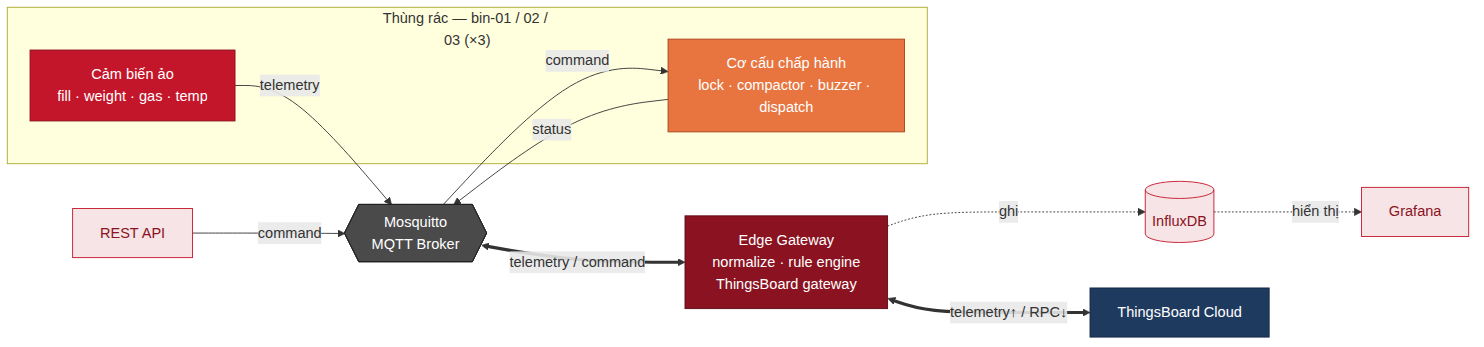
\includegraphics[width=\textwidth]{hinh1-kien-truc.png}
\caption{Kiến trúc lai của hệ thống: cảm biến và cơ cấu chấp hành giao tiếp qua Mosquitto; Edge Gateway chuẩn hóa dữ liệu, chạy rule engine, ghi InfluxDB và đồng bộ hai chiều với ThingsBoard Cloud; Grafana đọc InfluxDB để hiển thị; REST API cho phép truy vấn và điều khiển thủ công.}
\end{figure}

\textbf{Luồng dữ liệu chính:}
\begin{enumerate}[nosep]
    \item Cảm biến publish telemetry dạng JSON lên \texttt{waste/\{bin\}/sensor/telemetry} mỗi 5 đến 7 giây.
    \item Broker chuyển tiếp bản tin đến Edge Gateway. Gateway kiểm tra hợp lệ, chuẩn hóa rồi chạy rule engine.
    \item Gateway publish dữ liệu đã chuẩn hóa, sự kiện bất thường (nếu có), lệnh điều khiển xuống actuator, và ghi cả ba loại dữ liệu này vào InfluxDB.
    \item Actuator nhận lệnh, kiểm tra an toàn, cập nhật trạng thái nội bộ rồi publish lại trạng thái mới.
    \item Grafana đọc InfluxDB để hiển thị dashboard; một tiến trình riêng (\texttt{tb-gateway}) đẩy telemetry và sự kiện lên ThingsBoard, đồng thời chuyển lệnh RPC từ cloud thành command MQTT cục bộ.
\end{enumerate}

Điểm cốt lõi của kiến trúc này là tính lai: Edge Gateway vừa tự ra quyết định ngay tại biên, đảm bảo độ trễ thấp và vẫn hoạt động khi mất kết nối Internet, vừa gộp nhiều thùng rác vào một kết nối ThingsBoard Cloud duy nhất để giám sát tập trung. Mọi giao tiếp giữa các thiết bị đều đi qua broker MQTT, không thiết bị nào nối trực tiếp với thiết bị khác; broker đóng vai trò bus nội bộ tại biên, còn gateway là cầu nối duy nhất lên tầng lưu trữ và đám mây.

%=============================================================
\section{Cấu trúc project và danh sách service}
%=============================================================

\begin{lstlisting}[language=bash,frame=none,numbers=none]
iot-waste-management/
|-- docker-compose.yml
|-- .env.example
|-- mosquitto/config/mosquitto.conf
|-- virtual_sensor/      (sensor.py, Dockerfile, requirements.txt)
|-- virtual_actuator/    (actuator.py, Dockerfile, requirements.txt)
|-- iot_gateway/
|   |-- gateway.py            rule engine orchestrator + vong lap bao tri
|   |-- rule_engine.py        tap luat (ham thuan)
|   |-- state_store.py        trang thai + debounce + danh sach thu gom
|   |-- influx_writer.py      ghi InfluxDB
|   '-- tb_gateway.py         cau noi ThingsBoard
|-- gateway_api/         (api.py, FastAPI REST API)
|-- grafana/             (provisioning datasource + dashboard)
'-- docs/                (topic-design.md, bao cao, anh chup)
\end{lstlisting}

Bộ service khai báo trong \texttt{docker-compose.yml} gồm \texttt{mosquitto}, \texttt{influxdb}, \texttt{waste-gateway}, ba cặp \texttt{sensor-bin-01/02/03} và \texttt{actuator-bin-01/02/03}, \texttt{grafana}, \texttt{gateway-api}, và \texttt{tb-gateway} (chỉ khởi động khi kích hoạt profile \texttt{thingsboard}).

Mỗi service tự chứa mã nguồn, \texttt{requirements.txt} và \texttt{Dockerfile} riêng để Docker Compose build độc lập. Hai container \texttt{waste-gateway} và \texttt{tb-gateway} dùng chung codebase \texttt{iot\_gateway/} nhưng chạy hai entrypoint khác nhau, \texttt{gateway.py} và \texttt{tb\_gateway.py}. Về mặt logic, cả hai cùng thuộc thành phần Edge Gateway mà đề bài mô tả; việc tách thành hai process chỉ nhằm phân chia trách nhiệm giữa xử lý cục bộ và cầu nối cloud.

%=============================================================
\section{Thiết kế MQTT topic và message format}
%=============================================================

Cây topic được thiết kế theo từng thùng, mỗi thùng có một nhóm topic riêng:

\begin{lstlisting}[language=bash,frame=none,numbers=none]
waste/{bin_id}/
|-- sensor/telemetry      # fill/weight/gas/temp tho tu sensor
|-- sensor/reset          # gateway bao da thu gom, sensor reset
|-- actuator/command      # gateway gui lenh dieu khien
|-- actuator/status       # actuator phan hoi trang thai
|-- gateway/normalized    # du lieu da chuan hoa (gateway publish)
'-- gateway/event         # su kien bat thuong (gateway publish)
\end{lstlisting}

\textbf{Bản tin telemetry} (\texttt{waste/bin-01/sensor/telemetry}):
\begin{lstlisting}[language={}]
{
  "device_id": "sensor-bin-01", "area_id": "district-1", "bin_id": "bin-01",
  "fill_level": 88.0, "weight_kg": 70.4, "methane_ppm": 350.0,
  "temperature": 33.0, "lid_status": "closed", "tilt": false,
  "timestamp": "2026-06-10T10:00:00Z"
}
\end{lstlisting}

\textbf{Bản tin command} (\texttt{waste/bin-01/actuator/command}):
\begin{lstlisting}[language={}]
{ "bin_id": "bin-01", "target": "dispatch", "action": "on",
  "reason": "bin_full", "timestamp": "2026-06-10T10:00:05Z" }
\end{lstlisting}

Đặt \texttt{bin\_id} vào cấu trúc topic, không phải trong payload, cho phép gateway dùng một lệnh subscribe wildcard \texttt{waste/+/sensor/telemetry} để bắt telemetry của mọi thùng cùng lúc. Việc tách riêng ba nhóm \texttt{sensor/}, \texttt{actuator/} và \texttt{gateway/} giúp việc gỡ lỗi đơn giản hơn: chỉ cần subscribe một nhánh là xem được toàn bộ một loại dữ liệu. Mọi bản tin đều ở dạng JSON và luôn kèm \texttt{bin\_id} cùng \texttt{timestamp} để phục vụ truy vết.

%=============================================================
\section{Virtual Sensor: mô phỏng có xu hướng}
%=============================================================

Yêu cầu của đề bài là mức đầy phải biến đổi có xu hướng theo thời gian, không random độc lập giữa các chu kỳ, vì một thùng rác thật không thể tự vơi rồi đầy lại nếu không có xe đến thu gom.

\begin{lstlisting}[language=Python]
def _simulate_fill(self):
    if not self.locked:
        noise = random.gauss(0, 0.1)               # nhieu nho quanh xu huong
        self.fill_level += self._fill_rate + noise # fill_rate > 0 nen luon tang
        self.fill_level = max(0.0, min(100.0, self.fill_level))
    self.weight_kg = self.fill_level * KG_PER_FILL_PERCENT + random.gauss(0, 0.3)
\end{lstlisting}

Nồng độ methane có tương quan thuận với mức đầy theo công thức nền \texttt{base = 50 + fill\_level * 5}, kèm khoảng ba phần trăm xác suất mỗi chu kỳ xảy ra hiện tượng tăng đột biến từ ba trăm đến năm trăm ppm, mô phỏng túi khí bị vỡ. Nhiệt độ có thể leo thang từ hai mươi đến ba mươi lăm độ khi nồng độ methane vượt bốn trăm ppm, tạo thành đường dẫn dẫn tới sự kiện cháy. Thùng bị đánh dấu đổ nghiêng khi khối lượng vượt năm mươi lăm kilôgam. Khi nhận được lệnh \texttt{\{"action":"reset"\}} trên topic \texttt{sensor/reset}, sensor đặt mức đầy về khoảng 0,5 đến 3 phần trăm, mô phỏng việc vừa được thu gom.

Một chi tiết đáng chú ý được bổ sung trong quá trình hoàn thiện: sensor lắng nghe luôn topic \texttt{actuator/status} của chính thùng mình. Khi nắp bị khóa (\texttt{lock = on}, do quá tải), mức đầy và khối lượng sẽ ngừng tăng cho đến khi mở khóa hoặc thu gom xong, vì không ai có thể bỏ thêm rác vào một thùng đã khóa nắp. Nhờ vậy hành động khóa nắp có tác động thật lên mô phỏng, không chỉ là một cờ trạng thái hiển thị suông.

\begin{figure}[H]
\centering
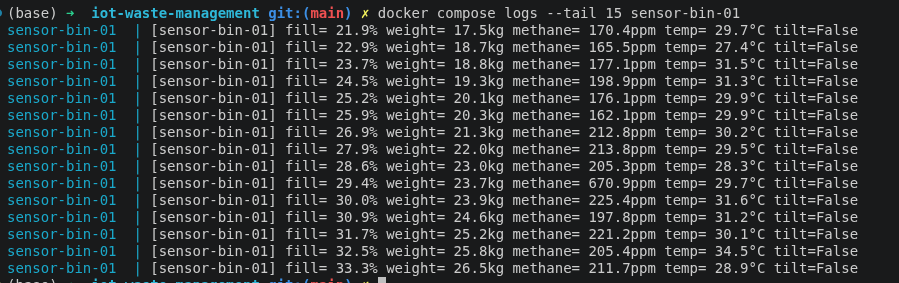
\includegraphics[width=0.85\textwidth]{hinh3-sensor-log.png}
\caption{Log của \texttt{sensor-bin-01} cho thấy mức đầy tăng dần qua từng chu kỳ, đúng yêu cầu mô phỏng có xu hướng.}
\end{figure}

Toàn bộ cấu hình của sensor, bao gồm \texttt{AREA\_ID}, \texttt{BIN\_ID} và \texttt{PUBLISH\_INTERVAL}, đều đọc từ biến môi trường theo nguyên tắc mười hai yếu tố (12-factor app), không hard-code trong mã nguồn. Hằng số \texttt{KG\_PER\_FILL\_PERCENT} được chọn bằng 0,8 một cách có chủ đích, đủ lớn để một thùng gần đầy vượt được cả ngưỡng quá tải (60 kg) và ngưỡng đổ nghiêng (55 kg); nếu chọn hằng số nhỏ hơn, hai tình huống này sẽ không bao giờ xảy ra và phần rule engine tương ứng không có cơ hội được kích hoạt.

%=============================================================
\section{Virtual Actuator và an toàn nhiều lớp}
%=============================================================

Actuator nhận lệnh, kiểm tra tính hợp lệ, áp dụng một lớp an toàn ngay tại thiết bị, rồi mới cập nhật trạng thái và phản hồi.

\begin{lstlisting}[language=Python]
if bin_id and bin_id != BIN_ID:                 # 1. lenh khong phai cua thung minh
    return
if target not in VALID_TARGETS:                 # 2. validate target
    _publish_error(client, f"invalid_target:{target}", reason); return
if action not in VALID_ACTIONS:                 # 3. validate action
    _publish_error(client, f"invalid_action:{action}", reason); return
# 4. SAFETY CHECK: cam nen rac khi dang bao chay
if target == "compactor" and action == "on" and state["buzzer"] == "on":
    _publish_error(client, "safety_block:compactor_during_fire_risk", reason); return
state[target] = action                          # 5. ap dung + publish status
client.publish(TOPIC_STATUS, json.dumps(build_status_payload()), qos=1)
\end{lstlisting}

\begin{figure}[H]
\centering
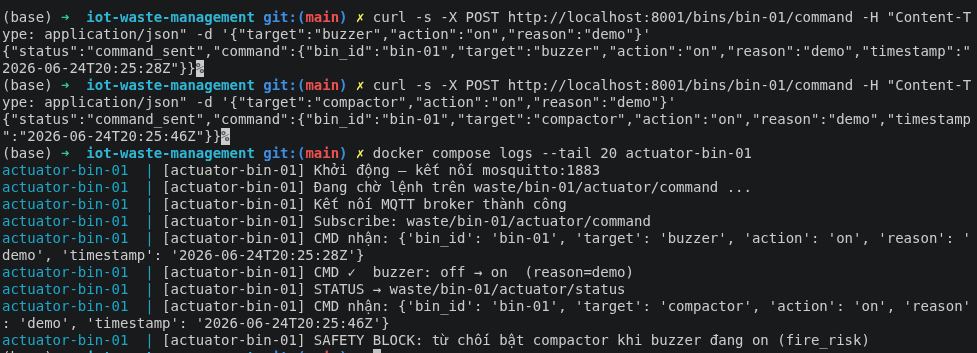
\includegraphics[width=0.85\textwidth]{hinh4-actuator-log.png}
\caption{Actuator thực thi lệnh hợp lệ và từ chối lệnh nguy hiểm bằng cơ chế safety block.}
\end{figure}

Quyết định an toàn được xử lý ngay tại thiết bị, không chờ gateway phản hồi, vì trong kịch bản cháy thực tế, độ trễ mạng dù nhỏ cũng có thể gây hậu quả nghiêm trọng. Đây là một ví dụ của nguyên tắc phòng vệ theo lớp: gateway đã chủ động tắt bộ nén rác khi phát hiện nguy cơ cháy, nhưng nếu vì lý do nào đó vẫn có lệnh nén rác gửi nhầm xuống, có thể do lỗi phần mềm hoặc do lệnh thủ công gửi qua REST API, actuator vẫn tự chặn lại. Một điểm thiết kế khác là actuator luôn publish toàn bộ trạng thái của bốn thiết bị sau mỗi lệnh, không chỉ gửi phần thay đổi, để gateway và ThingsBoard luôn đồng bộ kể cả khi một bản tin nào đó bị thất lạc trên đường truyền.

%=============================================================
\section{Edge Gateway: kiểm tra hợp lệ, chuẩn hóa và lưu trạng thái}
%=============================================================

Gateway là thành phần trung tâm của hệ thống, subscribe wildcard toàn bộ thùng, làm sạch dữ liệu đầu vào, lưu trạng thái mới nhất và duy trì danh sách thùng cần thu gom.

\begin{lstlisting}[language=Python]
for f in _REQUIRED_FIELDS:                       # du truong bat buoc
    if f not in raw: return None
if bin_from_topic and bin_id != bin_from_topic:  # bin_id khop topic, chong gia mao
    return None
datetime.strptime(raw["timestamp"], "%Y-%m-%dT%H:%M:%SZ")   # timestamp dung ISO-8601
fill = max(0.0, min(100.0, float(raw["fill_level"])))        # clamp + phan loai fill_status
\end{lstlisting}

\begin{lstlisting}[language=Python]
def update_telemetry(self, bin_id, normalized):     # luu trang thai moi nhat tung thung
    with self._lock:
        self.telemetry[bin_id] = normalized
        self._last_seen[bin_id] = time.monotonic()
def mark_for_collection(self, bin_id):              # them vao danh sach can thu gom
    with self._lock:
        self._collection.setdefault(bin_id, time.monotonic())
def due_for_collection(self, delay):                # thung da cho qua delay giay
    now = time.monotonic()
    with self._lock:
        return [b for b, ts in self._collection.items() if now - ts >= delay]
\end{lstlisting}

Khâu kiểm tra hợp lệ đóng vai trò tuyến phòng thủ đầu tiên: bản tin thiếu trường, sai định dạng timestamp, hoặc \texttt{bin\_id} trong payload không khớp với topic đều bị loại bỏ ngay, không làm gián đoạn vòng lặp MQTT đang chạy. Lớp \texttt{StateStore} bọc mọi thao tác đọc và ghi trong một khóa (lock), vì callback của thư viện MQTT chạy trên thread mạng riêng, còn vòng lặp bảo trì lại chạy trên thread chính; hai luồng này truy cập đồng thời vào cùng một vùng dữ liệu nên buộc phải đồng bộ hóa. Trạng thái mới nhất của từng thùng và danh sách thùng cần thu gom được lưu tại đây để phục vụ rule engine, cơ chế debounce lệnh điều khiển và việc mô phỏng vòng đời thu gom.

%=============================================================
\section{Rule Engine: tập luật phát hiện bất thường}
%=============================================================

Rule engine áp dụng một tập luật lên bản ghi telemetry đã chuẩn hóa, trả về sự kiện phát sinh và trạng thái mong muốn của từng cơ cấu chấp hành.

\begin{center}
\begin{tabular}{cllc}
\toprule
\textbf{Luật} & \textbf{Điều kiện} & \textbf{Sự kiện} & \textbf{Hành động} \\
\midrule
1 & fill\_level > 85 (>95: critical) & bin\_full & dispatch = on \\
2 & temperature > 60 & fire\_risk (critical) & buzzer = on, compactor = off \\
3 & methane\_ppm > 500 & gas\_alert (warning) & gợi ý thông khí \\
4 & weight\_kg > 60 & overweight (warning) & lock = on \\
5 & tilt = true & bin\_tilted (info) & lên lịch bảo trì \\
\bottomrule
\end{tabular}
\end{center}

\begin{lstlisting}[language=Python]
def evaluate(t: dict, th: Thresholds) -> dict:
    events, desired = {}, {}
    if fill > th.fill_dispatch:
        severity = "critical" if fill > th.fill_critical else "warning"
        events["bin_full"] = {...}
        desired["dispatch"] = "on"
    else:
        desired["dispatch"] = "off"     # het day, tu tat (level-based)
    return {"events": events, "desired": desired}
\end{lstlisting}

\begin{figure}[H]
\centering
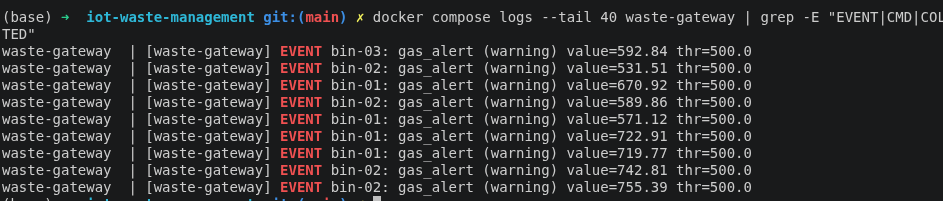
\includegraphics[width=0.9\textwidth]{hinh5-gateway-log.png}
\caption{Gateway ghi nhận sự kiện \texttt{bin\_full}, gửi lệnh \texttt{dispatch=on}, và sau đó publish lệnh reset khi xe mô phỏng đã đến thu gom.}
\end{figure}

Rule engine được thiết kế như một hàm thuần: cùng một đầu vào luôn cho ra cùng một đầu ra, không publish lên MQTT, không ghi cơ sở dữ liệu và không tự giữ trạng thái. Nhờ đặc điểm này, rule engine kiểm thử được hoàn toàn độc lập, không cần khởi động broker hay database thật. Thiết kế cũng tách bạch hai khái niệm dễ nhầm lẫn: trường \texttt{desired} mang tính theo mức, gateway dựa vào đó để debounce, chỉ gửi lệnh điều khiển khi trạng thái mong muốn thực sự thay đổi, tránh lặp lại mỗi chu kỳ; còn trường \texttt{events} mang tính cạnh, chỉ phát sinh đúng một lần tại thời điểm điều kiện chuyển từ sai sang đúng, giúp biểu đồ số lượng sự kiện theo thời gian trên Grafana phản ánh đúng ngữ nghĩa. Toàn bộ ngưỡng được đọc từ biến môi trường nên có thể chỉnh từ xa qua REST API hoặc ThingsBoard mà không cần sửa mã nguồn.

%=============================================================
\section{Ghi InfluxDB, vòng đời thu gom và phát hiện offline}
%=============================================================

Ba loại dữ liệu được ghi vào InfluxDB: \texttt{bin\_telemetry} với tag \texttt{area\_id}, \texttt{bin\_id} và field \texttt{fill\_level}, \texttt{weight\_kg}, \texttt{methane\_ppm}, \texttt{temperature}; \texttt{gateway\_events} với tag \texttt{bin\_id}, \texttt{event\_type}, \texttt{severity} và field \texttt{value}, \texttt{threshold}; \texttt{actuator\_status} với tag \texttt{bin\_id} và bốn field tương ứng bốn thiết bị, được mã hóa về dạng số 0 và 1 để Grafana vẽ được.

\begin{lstlisting}[language=Python]
for bin_id in store.due_for_collection(COLLECTION_DELAY):   # mo phong xe toi noi
    client.publish(f"waste/{bin_id}/sensor/reset", ...)     # sensor reset
    store.clear_collection(bin_id)
newly_offline, recovered = store.offline_transitions(SENSOR_OFFLINE_TIMEOUT)
for bin_id in newly_offline:                                 # qua han khong co telemetry
    client.publish(f"waste/{bin_id}/gateway/event", sensor_offline_payload)
\end{lstlisting}

\begin{figure}[H]
\centering
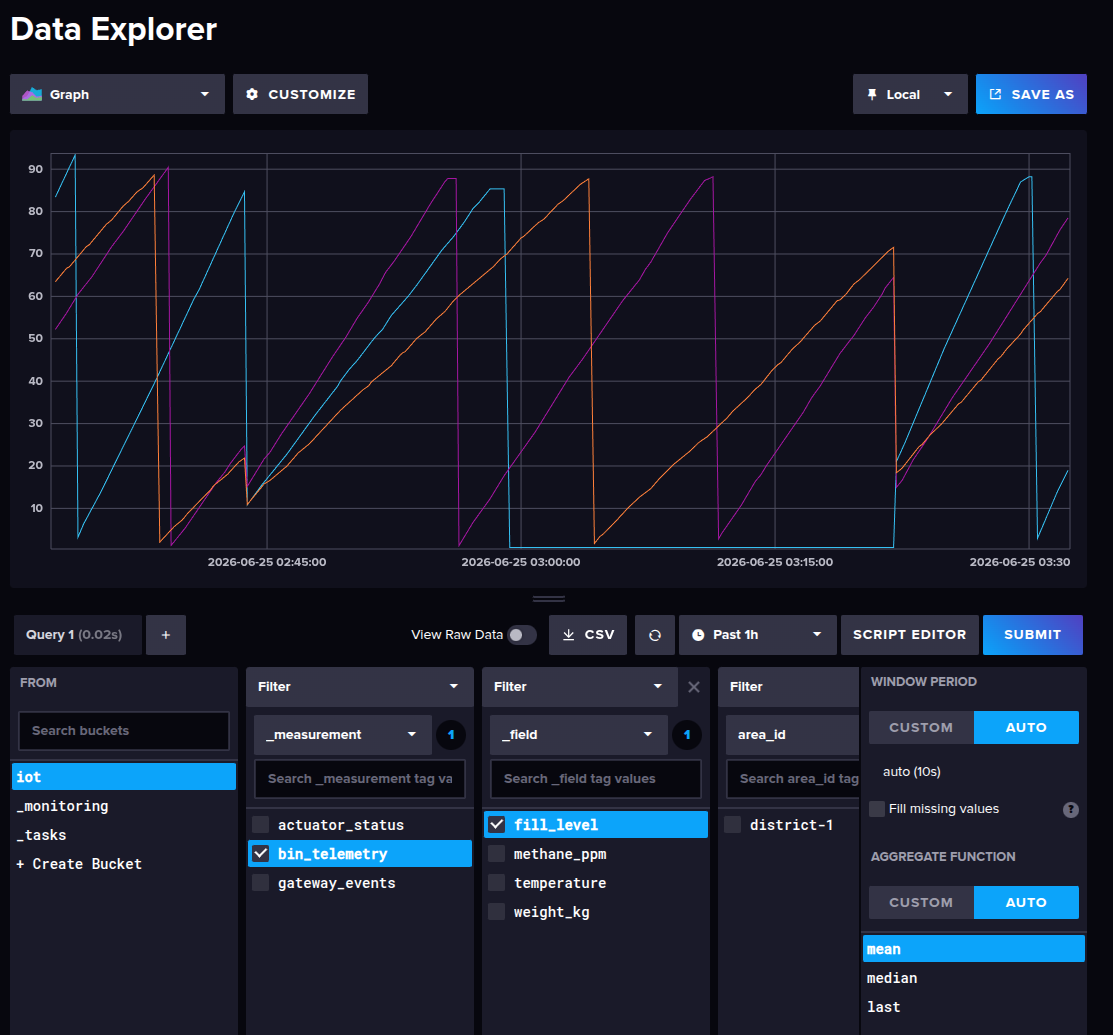
\includegraphics[width=0.95\textwidth]{hinh7-influxdb.png}
\caption{InfluxDB Data Explorer hiển thị measurement \texttt{bin\_telemetry} với trường \texttt{fill\_level} theo thời gian.}
\end{figure}

Một nguyên tắc thiết kế quan trọng là lỗi ghi InfluxDB không được phép làm gateway dừng hoạt động. Việc khởi tạo client InfluxDB được bọc trong khối thử bắt lỗi; nếu cơ sở dữ liệu tạm thời không sẵn sàng, gateway vẫn tiếp tục chạy ở chế độ không ghi, rule engine và việc điều khiển actuator không bị ảnh hưởng. Vòng đời thu gom khép kín theo trình tự: thùng đầy dẫn đến lệnh \texttt{dispatch=on}, thùng được đưa vào danh sách cần thu gom, sau một khoảng thời gian mô phỏng xe đến nơi, gateway publish lệnh reset, sensor đặt lại mức đầy gần 0 để bắt đầu một chu kỳ mới.

%=============================================================
\section{REST API}
%=============================================================

REST API đóng vai trò một lớp giao diện HTTP cho phía biên, cho phép truy vấn trạng thái và gửi lệnh điều khiển mà không cần nói trực tiếp giao thức MQTT.

\begin{lstlisting}[language={},frame=none,numbers=none]
GET  /health                  kiem tra service + danh sach bin
GET  /bins                    telemetry moi nhat moi thung (doc InfluxDB)
GET  /bins/{id}/state         telemetry + trang thai actuator
GET  /bins/{id}/events        su kien gan day
GET  /collection/route        danh sach thung can thu gom ngay bay gio
POST /bins/{id}/command       gui lenh thu cong
GET/POST /config              xem / dieu chinh nguong rule engine khi dang chay
\end{lstlisting}

\begin{figure}[H]
\centering
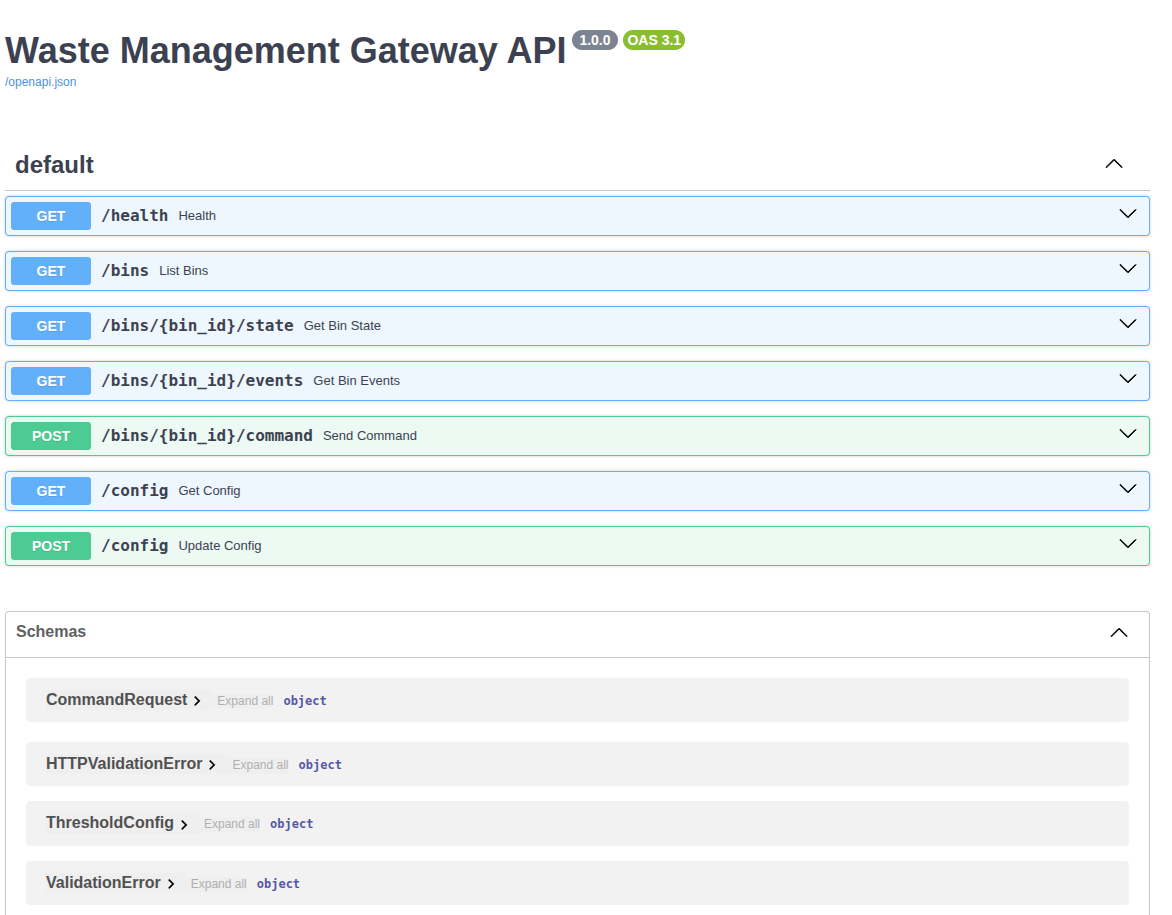
\includegraphics[width=0.95\textwidth]{hinh11-swagger.png}
\caption{Trang Swagger UI tại \texttt{http://localhost:8001/docs} liệt kê và cho phép thử trực tiếp các endpoint.}
\end{figure}

Các endpoint đọc trạng thái và sự kiện truy vấn trực tiếp vào InfluxDB bằng Flux, còn các endpoint điều khiển và cấu hình publish lệnh lên broker MQTT, không gọi trực tiếp vào gateway hay actuator. Dữ liệu đầu vào được kiểm tra bằng Pydantic, trả về mã lỗi 404 hoặc 400 theo đúng quy ước REST.

Đề bài liệt kê endpoint \texttt{GET /collection/route} làm danh sách thùng cần thu gom ngay tại thời điểm gọi. Hàm \texttt{collection\_route()} tương ứng đã có sẵn trong \texttt{state\_store.py}, nhưng vì \texttt{gateway-api} chạy trong một container riêng, không chia sẻ vùng nhớ với \texttt{waste-gateway}, nên không thể gọi trực tiếp hàm đó. Endpoint được hoàn thiện bằng cách suy ra danh sách từ giá trị \texttt{fill\_level} mới nhất của từng thùng trên InfluxDB, đúng cách mà panel Grafana "Thùng cần thu gom hiện tại" đã làm, sắp xếp giảm dần theo mức đầy để gợi ý thứ tự ưu tiên thu gom. Cách làm này tránh phải thêm một cơ chế chia sẻ trạng thái mới giữa hai container chỉ để phục vụ một endpoint.

Một lỗi khác chỉ lộ ra trong lúc tập demo: endpoint \texttt{GET /bins/\{id\}/state} có lúc báo \texttt{actuator} là \texttt{no\_data} dù thiết bị vẫn đang ở một trạng thái hợp lệ. Nguyên nhân nằm ở cửa sổ thời gian của câu truy vấn Flux. Hàm lấy telemetry mới nhất dùng \texttt{range(start: -5m)}, hợp lý vì sensor publish liên tục mỗi năm đến bảy giây nên luôn có dữ liệu trong năm phút gần nhất. Hàm lấy trạng thái actuator lại copy nguyên cửa sổ đó, nhưng actuator chỉ publish khi nhận lệnh mới, không publish định kỳ. Một thùng đã khóa nắp từ mười lăm phút trước, nếu không có lệnh nào khác xảy ra trong khoảng đó, sẽ bị API báo nhầm thành không có dữ liệu dù trạng thái khóa vẫn còn nguyên. Khi rà lại, nhóm em thấy panel Grafana "Trạng thái thiết bị theo thùng" đã dùng đúng cửa sổ hai mươi bốn giờ cho measurement \texttt{actuator\_status}, nên chỉ cần sửa REST API theo đúng cách đó là khớp lại. Đây là một minh chứng nữa cho việc dữ liệu theo chu kỳ và dữ liệu theo sự kiện cần chiến lược truy vấn khác nhau, dù cùng nằm trong một cơ sở dữ liệu.

%=============================================================
\section{Tích hợp ThingsBoard Cloud: uplink và RPC}
%=============================================================

Tiến trình \texttt{tb\_gateway.py} đóng vai trò cầu nối, sử dụng hai kết nối MQTT song song: một nối vào Mosquitto cục bộ, một nối lên \texttt{thingsboard.cloud} bằng ThingsBoard Gateway MQTT API.

\begin{lstlisting}[language=Python]
# UPLINK: doc du lieu chuan hoa tu broker, day len ThingsBoard
local_client.subscribe("waste/+/gateway/normalized")
tb_client.publish("v1/gateway/connect",  json.dumps({"device": bin_id}))
tb_client.publish("v1/gateway/telemetry", json.dumps({bin_id: [{"ts": ts, "values": values}]}))

# DOWNLINK: RPC tu ThingsBoard, chuyen thanh command MQTT cuc bo
def rpc_to_command(bin_id, method, params):     # setLock/setCompactor/setBuzzer/setDispatch
    return {"bin_id": bin_id, "target": RPC_METHOD_MAP[method],
            "action": rpc_action_from_params(params), "reason": "thingsboard_rpc"}
local_client.publish(f"waste/{bin_id}/actuator/command", json.dumps(command))
\end{lstlisting}

\begin{figure}[H]
\centering
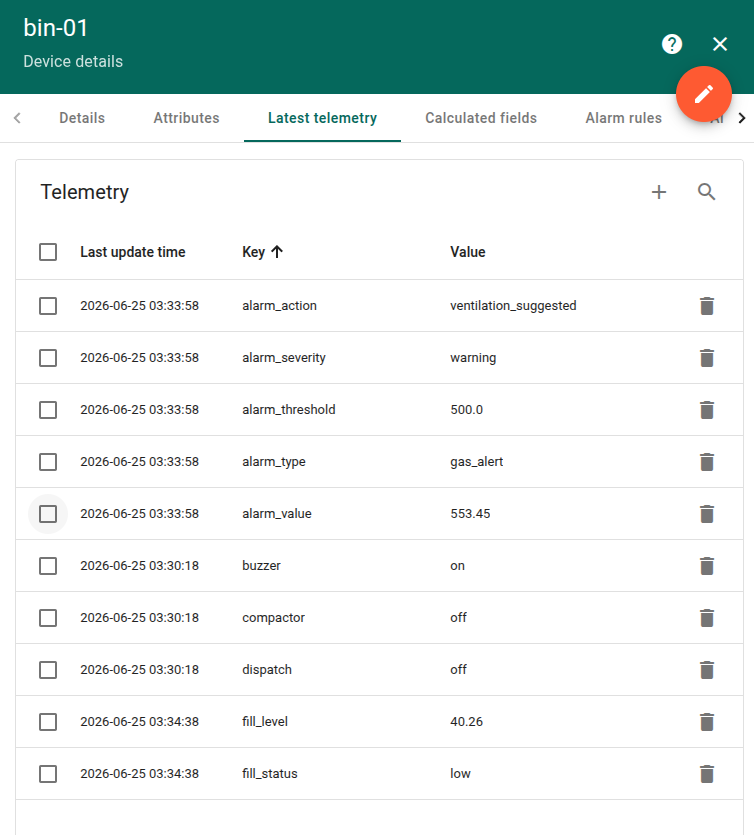
\includegraphics[width=0.7\textwidth]{hinh9-thingsboard-devices.png}
\caption{Ba thiết bị con bin-01, bin-02, bin-03 tự xuất hiện dưới gateway trên ThingsBoard Cloud; tab Latest telemetry cập nhật fill\_level, methane\_ppm và các trường khác theo thời gian thực.}
\end{figure}

\begin{figure}[H]
\centering
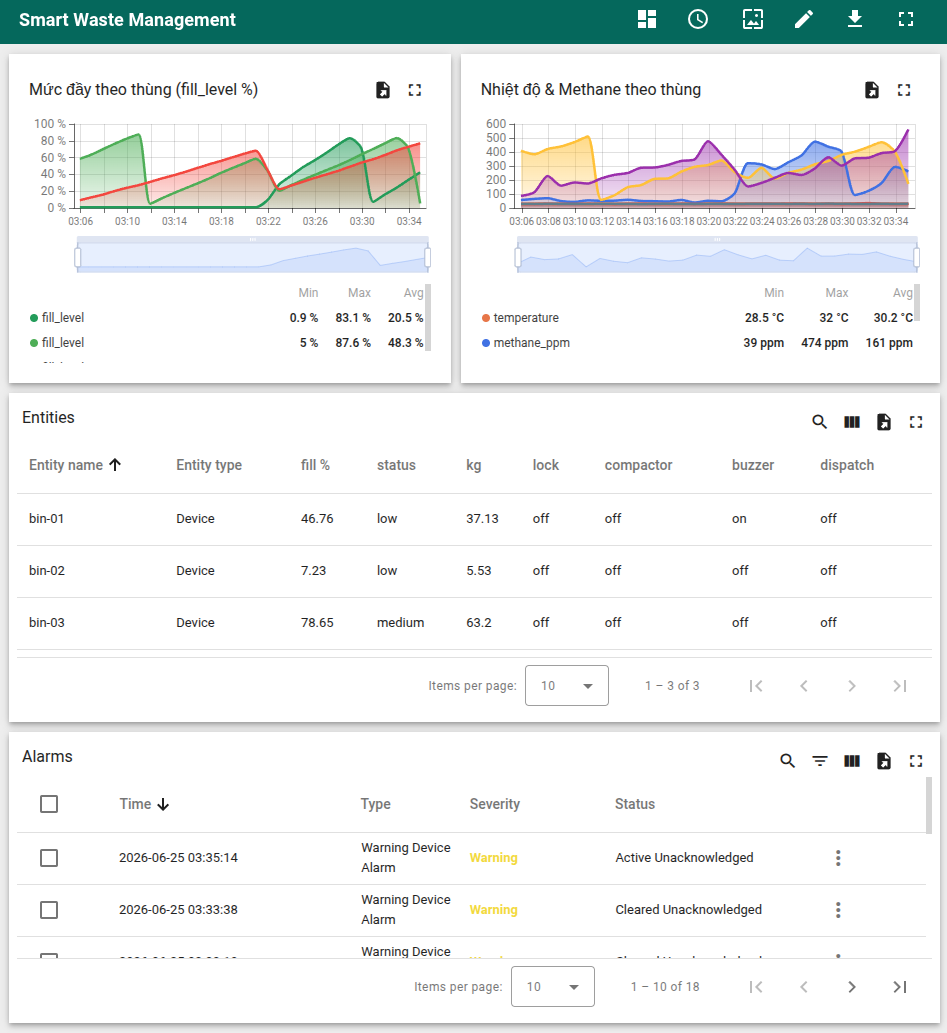
\includegraphics[width=0.75\textwidth]{hinh10-thingsboard-alarm.png}
\caption{Rule Chain trên ThingsBoard sinh Alarm mức Critical và Warning; dashboard có nút RPC điều khiển trực tiếp từ xa.}
\end{figure}

Bridge chỉ đẩy lên ThingsBoard dữ liệu đã được chuẩn hóa và sự kiện đã qua xử lý của gateway, không đẩy telemetry thô. Vai trò ThingsBoard gateway được tách thành một container riêng tên \texttt{tb-gateway}, dùng chung codebase với \texttt{waste-gateway} nhưng chạy độc lập; về bản chất, đây chính là phần ThingsBoard gateway của Edge Gateway mà đề bài yêu cầu.

Một sự cố đáng ghi lại trong quá trình tích hợp: phiên bản đầu gửi yêu cầu shared attributes lên topic \texttt{v1/gateway/attributes/request} với payload \texttt{\{"sharedKeys": ...\}}, là định dạng dành cho API của chính thiết bị gateway, không phải API xin thuộc tính của một sub-device. ThingsBoard nhận bản tin sai định dạng và ngắt kết nối ngay sau mỗi lần kết nối thành công, tạo ra một vòng lặp connect rồi disconnect lặp lại mỗi một đến hai giây. Lỗi này không bị unit test với mock phát hiện, chỉ lộ ra khi chạy thật trên Docker, vì bản chất của nó nằm ở giao tiếp thật với dịch vụ ThingsBoard Cloud. Sau khi đổi sang đúng topic \texttt{v1/devices/me/attributes/request/1}, kết nối ổn định trở lại.

%=============================================================
\section{Cấu hình ngưỡng rule engine khi đang chạy}
%=============================================================

Mục tiêu của phần này là cho phép đổi ngưỡng rule engine từ REST API hoặc từ ThingsBoard Shared Attributes mà không cần khởi động lại container.

\begin{lstlisting}[language={},frame=none,numbers=none]
REST POST /config          -+
                             +-> topic waste/gateway/config (retained)
ThingsBoard Shared Attr.   -+        -> gateway.handle_config_update()
                                         -> cap nhat THRESHOLDS ngay tuc thi
\end{lstlisting}

\begin{lstlisting}[language=Python]
def handle_config_update(payload):
    for env_key, value in payload.get("thresholds", {}).items():
        field = _THRESHOLD_ENV_TO_FIELD.get(env_key)
        if field:
            setattr(THRESHOLDS, field, float(value))   # co hieu luc tu telemetry ke tiep
\end{lstlisting}

Cả hai nguồn cấu hình cùng dùng một topic \texttt{waste/gateway/config}. Đối tượng \texttt{THRESHOLDS} là một dataclass có thể thay đổi giá trị (mutable), được dùng chung với hàm \texttt{evaluate()}, nên lệnh \texttt{setattr} có hiệu lực ngay từ bản telemetry kế tiếp. Bản tin sai định dạng hoặc giá trị không ép được về số thực sẽ bị bỏ qua một cách an toàn, không làm rule engine bị lỗi.

Tính năng này từng tồn tại trên giấy nhưng không có tác dụng thật: cả hai nguồn đều publish lên đúng topic, song ban đầu không thành phần nào subscribe topic đó. Sau khi bổ sung phần subscribe và xử lý ở gateway, một bộ kiểm thử đơn vị đã chứng minh việc hạ ngưỡng nhiệt độ cháy qua đúng đường dữ liệu này làm cùng một bản ghi telemetry chuyển từ trạng thái an toàn sang trạng thái \texttt{fire\_risk} ngay lập tức.

%=============================================================
\section{Grafana Dashboard}
%=============================================================

InfluxDB được khai báo làm data source cho Grafana thông qua cấu hình provisioning tự động, gọi vào InfluxDB bằng địa chỉ \texttt{http://influxdb:8086}, dùng tên service thay vì \texttt{localhost}, với ngôn ngữ truy vấn Flux.

Dashboard gồm tám panel, đủ cả sáu nhóm mà đề bài yêu cầu: mức đầy theo thời gian cho từng thùng kèm đường ngưỡng thu gom 85 phần trăm; khối lượng theo thời gian cho từng thùng; nhiệt độ và nồng độ methane theo thùng, mỗi đại lượng một panel riêng kèm đường ngưỡng cảnh báo; trạng thái bốn thiết bị chấp hành theo từng thùng dưới dạng bảng; số lượng sự kiện theo thời gian tách theo loại sự kiện; bảng các thùng đang cần thu gom ngay tại thời điểm xem, suy ra từ mức đầy mới nhất vượt 85 phần trăm; và bảng sự kiện gần nhất kèm mức độ nghiêm trọng.

\begin{figure}[H]
\centering
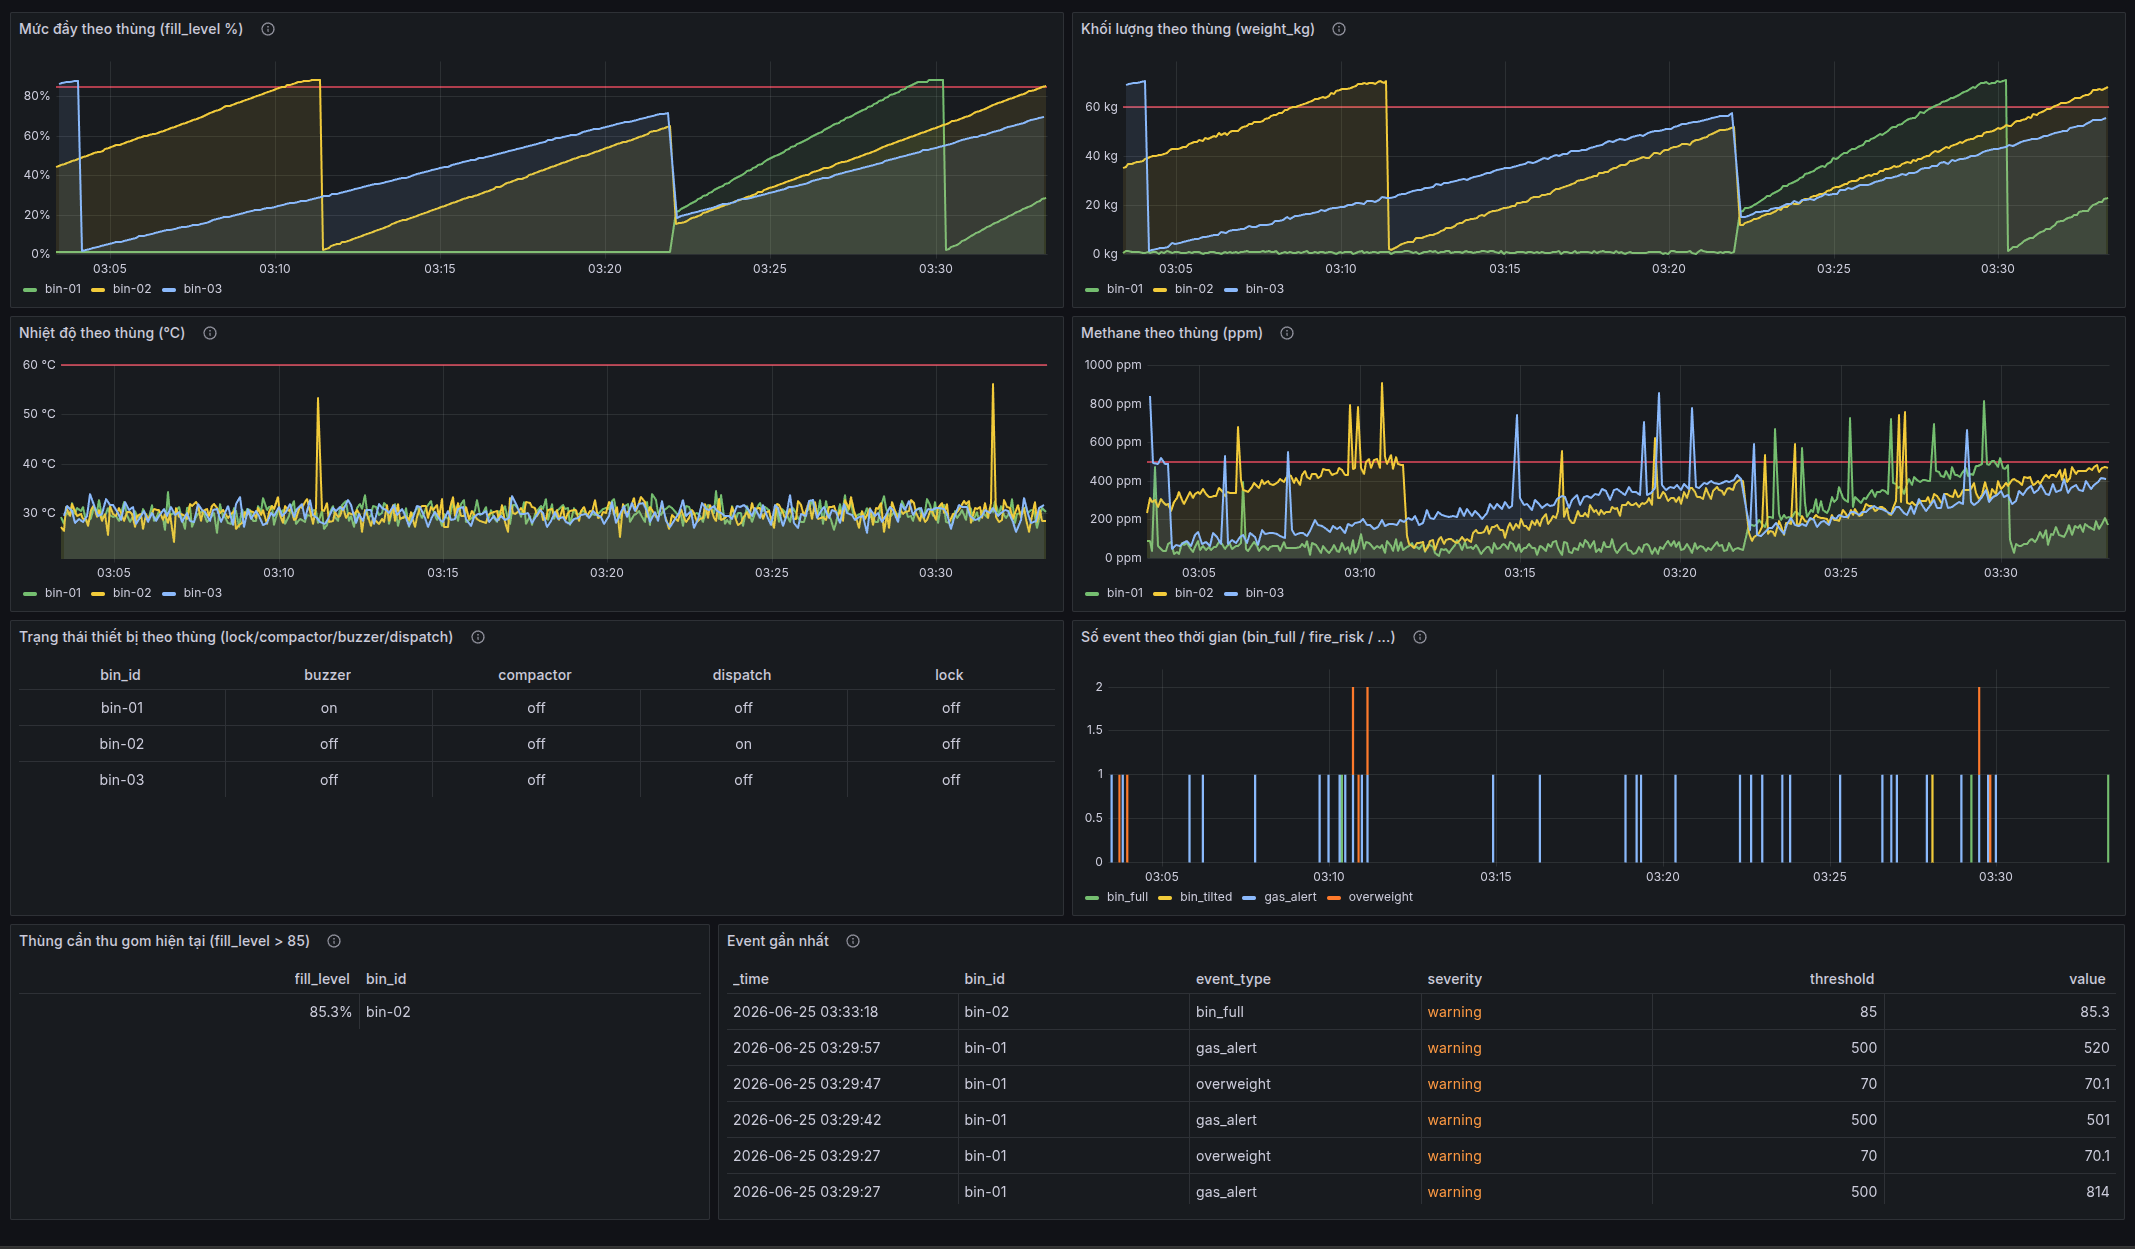
\includegraphics[width=\textwidth]{hinh8-grafana.png}
\caption{Dashboard Grafana hiển thị mức đầy, nhiệt độ và methane, trạng thái thiết bị, cùng số lượng sự kiện theo thời gian thực của ba thùng rác.}
\end{figure}

Dashboard thể hiện rõ mối liên hệ nhân quả trong hệ thống: khi mức đầy của một thùng vượt ngưỡng, sự kiện \texttt{bin\_full} xuất hiện ngay trên panel sự kiện và tín hiệu \texttt{dispatch} của thùng đó chuyển sang trạng thái bật. Toàn bộ chuỗi xử lý từ thiết bị, qua MQTT, qua gateway, vào InfluxDB, đến Grafana đều thông suốt và quan sát được trực tiếp trên một màn hình duy nhất.

%=============================================================
\section{Triển khai bằng Docker Compose}
%=============================================================

\begin{lstlisting}[language=bash]
cp .env.example .env
docker compose up -d --build
docker compose --profile thingsboard up -d --build tb-gateway
docker compose ps
\end{lstlisting}

\begin{figure}[H]
\centering
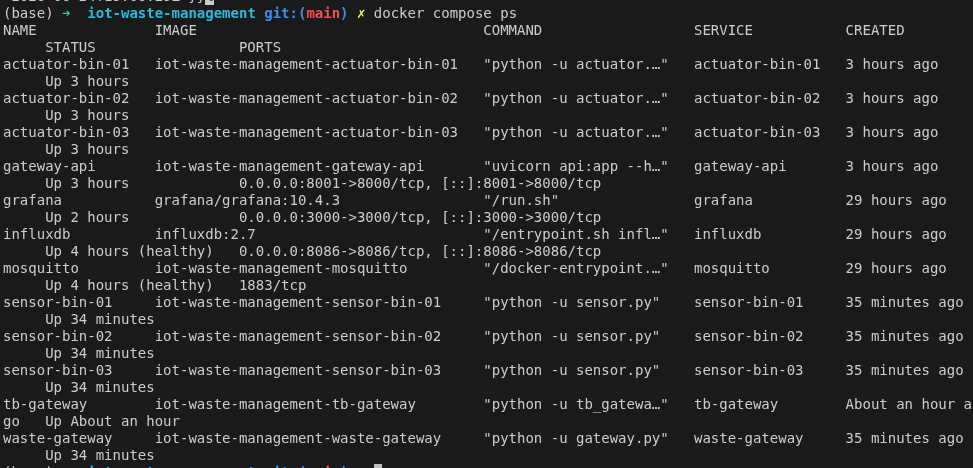
\includegraphics[width=0.95\textwidth]{hinh2-compose-ps.png}
\caption{Kết quả \texttt{docker compose ps}: mosquitto, influxdb, waste-gateway, ba sensor, ba actuator, grafana và gateway-api đều ở trạng thái Up.}
\end{figure}

Một lệnh duy nhất dựng toàn bộ hệ thống. Mọi tham số cấu hình đọc từ biến môi trường và file \texttt{.env}, theo đúng nguyên tắc mười hai yếu tố (xem Phụ lục A để biết đầy đủ ý nghĩa từng biến). Các service gọi nhau bằng tên service trong mạng \texttt{iot\_net} do Docker Compose tạo ra, tuyệt đối không dùng \texttt{localhost}. Mosquitto và InfluxDB có healthcheck riêng; mọi service đều đặt chính sách \texttt{restart: unless-stopped}; dữ liệu InfluxDB và Grafana được giữ lại qua named volume kể cả khi container bị xóa và tạo lại. Thành phần ThingsBoard được tách theo profile riêng để chỉ khởi động khi đã có token hợp lệ, tránh lỗi không cần thiết khi chưa cấu hình ThingsBoard.

Khi cần dừng hệ thống, hai lệnh sau được dùng tùy mục đích:
\begin{lstlisting}[language=bash]
docker compose down         # dung container, giu lai volume du lieu
docker compose down -v      # xoa ca volume (mat du lieu InfluxDB/Grafana)
\end{lstlisting}

%=============================================================
\section{Kiểm thử hệ thống}
%=============================================================

\begin{lstlisting}[language=bash]
docker exec mosquitto mosquitto_sub -t "waste/+/sensor/telemetry" -v
docker exec mosquitto mosquitto_sub -t "waste/+/gateway/event" -v
\end{lstlisting}

\begin{figure}[H]
\centering
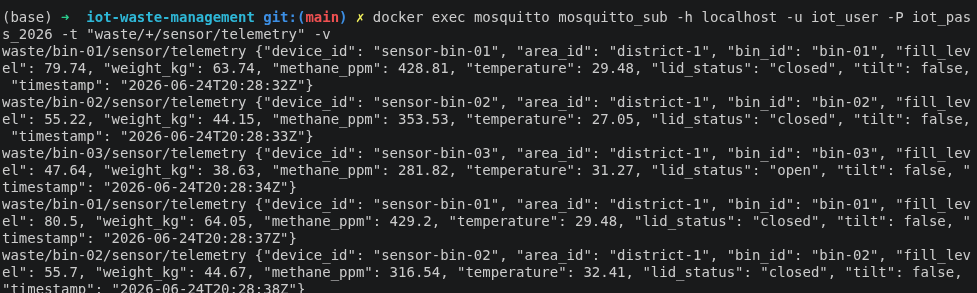
\includegraphics[width=0.95\textwidth]{hinh6-mosquitto-sub.png}
\caption{Subscriber nhận đúng bản tin JSON telemetry từ cả ba thùng rác.}
\end{figure}

Song song với kiểm thử thủ công bằng \texttt{mosquitto\_sub}, hệ thống có một bộ unit test chạy bằng \texttt{unittest} của Python, không cần Docker, broker hay database thật:

\begin{lstlisting}[language=bash]
python -m unittest discover -s iot_gateway -p "test_*.py" -v
python -m unittest discover -s gateway_api -p "test_*.py" -v
python -m unittest discover -s virtual_sensor -p "test_*.py" -v
\end{lstlisting}

Phạm vi kiểm thử bao gồm rule engine và state store với các trường hợp debounce lệnh, phát hiện cạnh sự kiện và vòng đời thu gom; cầu nối ThingsBoard với việc chuyển đổi RPC, đóng gói payload telemetry và alarm, xử lý shared attributes; REST API với việc kiểm tra đầu vào, mã lỗi 404 và 400, gửi lệnh và đọc InfluxDB ở dạng giả lập; và hành vi khóa nắp của virtual sensor. Tổng số hơn sáu mươi sáu test, toàn bộ đều đạt.

\begin{figure}[H]
\centering
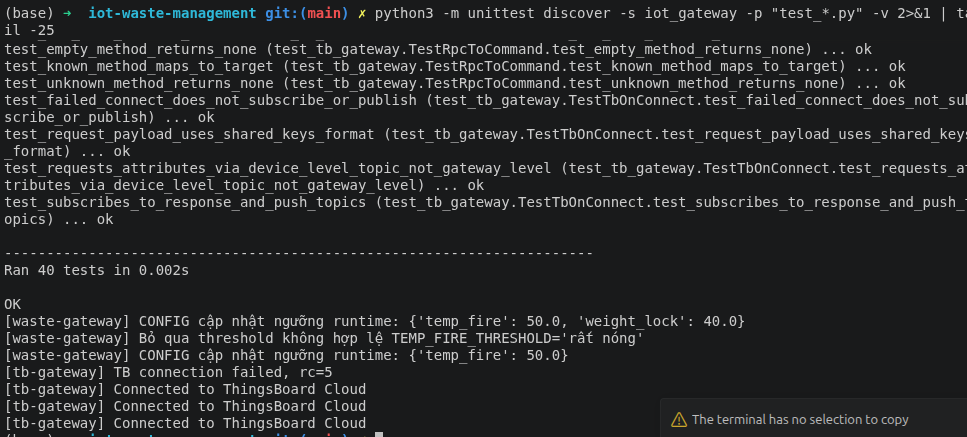
\includegraphics[width=0.9\textwidth]{hinh12-unittest.png}
\caption{Kết quả chạy unit test cho rule engine, tb\_gateway và REST API, tất cả đều PASS.}
\end{figure}

Triết lý kiểm thử xuyên suốt là tách phần logic thuần ra khỏi phần vào ra (I/O): các hàm tính toán trong rule engine và các hàm chuyển đổi dữ liệu trong tb\_gateway đều không gọi mạng, nên kiểm thử được độc lập, nhanh và không phụ thuộc môi trường. Công cụ \texttt{mosquitto\_sub} vẫn giữ vai trò là cách nhanh nhất để xác nhận luồng MQTT đang chạy đúng, trước khi đi sâu kiểm tra InfluxDB hay Grafana.

%=============================================================
\section{Khó khăn, bài học và hướng phát triển}
%=============================================================

\begin{itemize}
    \item \textbf{Kết nối ThingsBoard chập chờn.} Như đã trình bày ở Mục 11, việc gửi sai định dạng API yêu cầu shared attributes khiến ThingsBoard ngắt kết nối liên tục. Bài học rút ra là phải nắm chính xác đặc tả của từng API, không suy đoán theo cảm tính dù hai API trông tương tự nhau.
    \item \textbf{Lỗi chỉ lộ ra khi chạy thật.} Bộ unit test dùng mock không phát hiện được lỗi trên, vì nó nằm ở tầng giao tiếp thật với dịch vụ bên ngoài. Điều này cho thấy kiểm thử đơn vị và kiểm thử tích hợp bổ sung cho nhau, không thể thay thế nhau hoàn toàn.
    \item \textbf{Tính năng tồn tại trên giấy.} Topic \texttt{waste/gateway/config} từng được publish đầy đủ nhưng không có thành phần nào subscribe, khiến tính năng chỉnh ngưỡng runtime không có tác dụng thật dù từng dòng code liên quan đều đúng. Bài học là kiểm tra đầu cuối toàn bộ luồng dữ liệu quan trọng hơn việc kiểm tra từng module riêng lẻ.
    \item \textbf{Dừng tiến trình an toàn.} Lệnh \texttt{docker stop} gửi tín hiệu SIGTERM, không phải SIGINT mà chương trình ban đầu chỉ bắt qua \texttt{KeyboardInterrupt}. Nhóm đã bổ sung xử lý tín hiệu SIGTERM để đảm bảo kết nối MQTT lên ThingsBoard được đóng sạch trước khi container dừng, tránh để lại một phiên kết nối "ma" gây nhiễu cho lần khởi động kế tiếp.
    \item \textbf{Hằng số mô phỏng chưa phù hợp.} Hằng số \texttt{KG\_PER\_FILL\_PERCENT} ban đầu được chọn quá nhỏ, khiến hai sự kiện \texttt{overweight} và \texttt{bin\_tilted} không bao giờ xảy ra trong thực tế mô phỏng. Sau khi tăng giá trị này lên 0,8, rule engine kích hoạt được đúng như thiết kế.
    \item \textbf{Nhầm cửa sổ truy vấn giữa dữ liệu định kỳ và dữ liệu theo sự kiện.} Phát hiện trong buổi tập demo, đã trình bày chi tiết ở Mục 9: copy nguyên cửa sổ \texttt{-5m} từ hàm lấy telemetry sang hàm lấy trạng thái actuator khiến API báo nhầm trạng thái hợp lệ thành không có dữ liệu. Bài học là không nên sao chép tham số truy vấn giữa hai loại dữ liệu có nhịp publish khác nhau mà không xem lại từng trường hợp.
\end{itemize}

Hướng phát triển tiếp theo gồm bảo mật kết nối MQTT bằng TLS kết hợp xác thực thiết bị chặt chẽ hơn, dự báo thời điểm thùng đầy dựa trên tốc độ tăng mức đầy quan sát được, mở rộng thuật toán tối ưu lộ trình thu gom cho quy mô nhiều khu vực và nhiều gateway, cùng việc nối thêm kênh thông báo qua email hoặc Telegram khi Alarm trên ThingsBoard chuyển sang mức nguy cấp.

%=============================================================
\section{Trả lời câu hỏi bắt buộc trong báo cáo}
%=============================================================

\begin{enumerate}
    \item \textbf{Vì sao thu gom theo nhu cầu hiệu quả hơn lịch cố định? Edge gateway hỗ trợ thế nào?}

    Lịch cố định không biết thùng nào thực sự đầy nên vừa lãng phí khi đi thu những thùng còn trống, vừa rủi ro khi thùng tràn đúng vào lúc giữa hai chuyến thu gom. Thu gom theo nhu cầu chỉ điều xe khi mức đầy thực tế vượt ngưỡng, dựa trên dữ liệu thời gian thực thay vì lịch trình cố định từ trước. Edge gateway hỗ trợ bằng cách giám sát liên tục mọi thùng, chạy rule engine để phát hiện thùng đã đầy, duy trì một danh sách các thùng cần thu gom, và phát tín hiệu điều xe ngay tại biên mà không phải chờ một quyết định từ trên cloud.

    \item \textbf{Nhóm thiết kế topic và message format cho thùng rác thông minh thế nào?}

    Topic được phân cấp theo mẫu \texttt{waste/\{bin\_id\}/\{nhóm\}/\{loại\}}, với \texttt{bin\_id} nằm ngay trong cấu trúc topic để gateway có thể subscribe wildcard một lần cho mọi thùng. Ba nhóm con \texttt{sensor/}, \texttt{actuator/} và \texttt{gateway/} được tách riêng để dễ theo dõi từng loại dữ liệu. Mọi bản tin đều là JSON, luôn có \texttt{bin\_id} và \texttt{timestamp}; telemetry gồm các trường mức đầy, khối lượng, nồng độ methane, nhiệt độ, trạng thái nắp và cờ đổ nghiêng, như trình bày ở Mục 4.

    \item \textbf{Rule engine xử lý tình huống đầy, cháy, quá tải theo những luật nào?}

    Năm luật đã trình bày ở Mục 7: mức đầy vượt 85 phần trăm bật tín hiệu điều xe và sinh sự kiện \texttt{bin\_full}, vượt 95 phần trăm thì sự kiện này nâng lên mức critical; nhiệt độ vượt 60 độ bật còi đồng thời tắt bộ nén rác, sinh sự kiện \texttt{fire\_risk} ở mức critical; nồng độ methane vượt 500 ppm sinh sự kiện \texttt{gas\_alert}; khối lượng vượt 60 kilôgam khóa nắp và sinh sự kiện \texttt{overweight}; thùng bị đổ nghiêng sinh sự kiện \texttt{bin\_tilted} ở mức info để đưa vào lịch bảo trì. Mỗi sự kiện đều mang một mức độ nghiêm trọng rõ ràng, từ info, warning đến critical.

    \item \textbf{Gateway duy trì danh sách thùng cần thu gom ra sao?}

    Khi rule engine xác định một thùng cần điều xe, gateway gọi hàm \texttt{mark\_for\_collection} để lưu thời điểm thùng được đưa vào danh sách. Vòng lặp bảo trì chạy định kỳ, gọi hàm \texttt{due\_for\_collection} để mô phỏng thời điểm xe thu gom đến nơi, publish lệnh reset cho sensor, rồi gọi \texttt{clear\_collection} để đưa thùng ra khỏi danh sách. Hàm \texttt{collection\_route} trả về danh sách đã sắp theo thời gian chờ lâu nhất, gợi ý thứ tự nên thu gom trước.

    \item \textbf{Gateway đóng vai trò ThingsBoard Gateway như thế nào?}

    Gateway sử dụng ThingsBoard Gateway MQTT API: kết nối từng thùng như một sub-device thông qua topic \texttt{v1/gateway/connect}, đẩy telemetry của nhiều thùng cùng lúc qua \texttt{v1/gateway/telemetry}, nhận lệnh điều khiển qua \texttt{v1/gateway/rpc} rồi chuyển thành command MQTT cục bộ, và nhận Shared Attributes từ cloud để cập nhật ngưỡng rule engine. Trong cách triển khai của nhóm, vai trò này chạy ở một container riêng tên \texttt{tb-gateway}, đọc dữ liệu đã chuẩn hóa từ broker cục bộ rồi mới đẩy lên cloud, như trình bày ở Mục 10.

    \item \textbf{Vì sao một số quyết định, ví dụ báo cháy, nên xử lý ngay tại edge?}

    Vì độ trễ khứ hồi lên cloud, dù chỉ vài trăm milli giây, cũng có thể gây hậu quả nghiêm trọng trong một tình huống cháy. Quyết định an toàn như bật còi và cấm nén rác được xử lý ngay tại gateway và actuator theo nguyên tắc phòng vệ nhiều lớp, nên hệ thống vẫn hoạt động đúng kể cả khi mất kết nối Internet hoàn toàn.

    \item \textbf{Vì sao container không nên dùng \texttt{localhost} để gọi service khác?}

    Mỗi container có một network namespace riêng biệt, nên \texttt{localhost} bên trong một container chỉ trỏ về chính container đó, không trỏ tới container khác dù chạy trên cùng máy host. Khi các container cùng nằm trong một mạng Docker Compose, Docker cung cấp cơ chế phân giải tên dựa trên tên service, cho phép gọi \texttt{mosquitto} hay \texttt{influxdb} và tự động được dẫn tới địa chỉ IP nội bộ tương ứng.

    \item \textbf{Muốn mở rộng tối ưu lộ trình thu gom toàn thành phố trên ThingsBoard, cần thêm gì?}

    Cần mở rộng sang nhiều khu vực với nhiều gateway, mỗi gateway dùng một token riêng; gắn tọa độ địa lý cho từng thùng để hiển thị trên bản đồ của ThingsBoard; bổ sung một dịch vụ tối ưu tuyến đường, nhận danh sách thùng cần thu gom làm đầu vào và trả về thứ tự ghé thăm tối ưu cho từng xe; cùng với một Rule Chain ở mức cao hơn để tổng hợp dữ liệu từ nhiều khu vực và điều phối cảnh báo tập trung.
\end{enumerate}

%=============================================================
\section{Kết luận}
%=============================================================

Nhóm em đã hoàn thiện một hệ thống IoT ảo hóa đầu cuối cho bài toán quản lý thùng rác thông minh, từ tầng thiết bị giả lập đến tầng xử lý tại biên, lưu trữ thời gian thực và giám sát trên cả Grafana và ThingsBoard Cloud. Hệ thống vận hành tự động: phát hiện thùng đầy thì điều xe, phát hiện nguy cơ cháy thì bật còi và khóa bộ nén rác, phát hiện quá tải thì khóa nắp, đồng thời vẫn cho phép can thiệp thủ công qua REST API hoặc lệnh RPC từ xa.

Quá trình thực hiện cũng cho thấy giá trị của việc kiểm thử ở nhiều tầng khác nhau. Nhiều lỗi tinh vi, từ sai định dạng API của ThingsBoard đến một tính năng tưởng đã hoàn chỉnh nhưng thực ra không ai lắng nghe, chỉ lộ ra khi toàn bộ hệ thống được chạy thật trên Docker, chứ không thể phát hiện chỉ bằng unit test. Đây là một bài học thực tế về sự khác biệt giữa việc một đoạn mã chạy đúng cú pháp và việc cả hệ thống hoạt động đúng như thiết kế.

\appendix
%=============================================================
\section{Bảng biến môi trường đầy đủ}
%=============================================================

Toàn bộ tham số của hệ thống đọc từ file \texttt{.env}, không hard-code trong mã nguồn. Bảng dưới đây liệt kê đầy đủ các biến khai báo trong \texttt{.env.example} cùng ý nghĩa và giá trị mặc định.

\small
\renewcommand{\arraystretch}{1.2}
\begin{longtable}{p{4.8cm}p{2.2cm}p{7.5cm}}
\toprule
\textbf{Biến} & \textbf{Mặc định} & \textbf{Ý nghĩa} \\
\midrule
\endhead
\bottomrule
\endlastfoot
\multicolumn{3}{l}{\textit{MQTT Broker}} \\
MQTT\_\allowbreak BROKER & mosquitto & Tên service broker, dùng để các container khác kết nối \\
MQTT\_\allowbreak PORT & 1883 & Cổng MQTT \\
MQTT\_\allowbreak USER & iot\_\allowbreak user & Tài khoản xác thực với Mosquitto \\
MQTT\_\allowbreak PASS & iot\_\allowbreak pass\_\allowbreak 2026 & Mật khẩu xác thực với Mosquitto \\
\multicolumn{3}{l}{\textit{Định danh khu vực và gateway}} \\
AREA\_\allowbreak ID & district-1 & Mã khu vực địa lý, gắn vào tag InfluxDB \\
GATEWAY\_\allowbreak ID & waste-gateway & Tên định danh của edge gateway trên MQTT \\
\multicolumn{3}{l}{\textit{Chu kỳ publish của sensor}} \\
PUBLISH\_\allowbreak INTERVAL & 5 & Chu kỳ publish telemetry, áp dụng cho bin-01 và bin-02 (giây) \\
PUBLISH\_\allowbreak INTERVAL\_\allowbreak BIN03 & 7 & Chu kỳ riêng của bin-03, để ba thùng không đồng pha \\
\multicolumn{3}{l}{\textit{ThingsBoard Cloud}} \\
TB\_\allowbreak HOST & thingsboard.\allowbreak cloud & Địa chỉ MQTT broker của ThingsBoard \\
TB\_\allowbreak PORT & 1883 & Cổng MQTT của ThingsBoard \\
TB\_\allowbreak GATEWAY\_\allowbreak TOKEN & (rỗng) & Access token của Gateway Device, mỗi người tự tạo riêng \\
\multicolumn{3}{l}{\textit{InfluxDB}} \\
INFLUXDB\_\allowbreak URL & http://\allowbreak influxdb:\allowbreak 8086 & Địa chỉ HTTP của InfluxDB, dùng tên service \\
INFLUXDB\_\allowbreak TOKEN & dev-token-change-me & Token đọc/ghi InfluxDB \\
INFLUXDB\_\allowbreak ORG & hust & Organization trong InfluxDB \\
INFLUXDB\_\allowbreak BUCKET & iot & Bucket lưu toàn bộ measurement time-series \\
INFLUXDB\_\allowbreak USERNAME & admin & Tài khoản đăng nhập giao diện InfluxDB \\
INFLUXDB\_\allowbreak PASSWORD & admin12345 & Mật khẩu đăng nhập giao diện InfluxDB \\
\multicolumn{3}{l}{\textit{Ngưỡng rule engine}} \\
FILL\_\allowbreak DISPATCH\_\allowbreak THRESHOLD & 85 & Mức đầy (\%) bắt đầu điều xe thu gom \\
FILL\_\allowbreak CRITICAL\_\allowbreak THRESHOLD & 95 & Mức đầy (\%) nâng sự kiện bin\_\allowbreak full lên critical \\
TEMP\_\allowbreak FIRE\_\allowbreak THRESHOLD & 60 & Nhiệt độ (°C) coi là có nguy cơ cháy \\
METHANE\_\allowbreak ALERT\_\allowbreak THRESHOLD & 500 & Nồng độ methane (ppm) phát cảnh báo khí \\
WEIGHT\_\allowbreak LOCK\_\allowbreak THRESHOLD & 70 & Khối lượng (kg) kích hoạt khóa nắp chống quá tải \\
SENSOR\_\allowbreak OFFLINE\_\allowbreak TIMEOUT & 30 & Thời gian (giây) không nhận telemetry thì coi sensor offline \\
COLLECTION\_\allowbreak DELAY & 60 & Thời gian (giây) mô phỏng xe đến nơi sau khi vào danh sách thu gom \\
\multicolumn{3}{l}{\textit{REST API và Grafana}} \\
BIN\_\allowbreak IDS & bin-01,bin-02,bin-03 & Danh sách bin mà REST API lặp qua khi truy vấn \\
GRAFANA\_\allowbreak USER & admin & Tài khoản đăng nhập Grafana \\
GRAFANA\_\allowbreak PASSWORD & admin & Mật khẩu đăng nhập Grafana \\
\end{longtable}
\normalsize
\renewcommand{\arraystretch}{1}

%=============================================================
\section{Kịch bản nguy cơ cháy minh họa}
%=============================================================

Phụ lục này trình bày chi tiết một lượt xử lý đầy đủ của kịch bản nguy cơ cháy, từ lúc sensor sinh ra giá trị bất thường đến lúc actuator phản hồi, để làm rõ cách các thành phần phối hợp với nhau theo đúng nguyên tắc phòng vệ nhiều lớp đã nói ở Mục 5 và Mục 7.

\begin{enumerate}[nosep]
    \item \textbf{Sensor phát hiện bất thường.} Theo công thức mô phỏng ở Mục 4, khi \texttt{methane\_ppm} vượt 400 ppm, có hai phần trăm xác suất mỗi chu kỳ nhiệt độ leo thang thêm hai mươi đến ba mươi lăm độ. Một lần leo thang thực tế quan sát được: \texttt{temperature = 72.5}, \texttt{methane\_ppm = 520.0}.
    \item \textbf{Gateway chạy rule engine.} Giá trị 72,5 độ vượt ngưỡng \texttt{TEMP\_FIRE\_THRESHOLD} bằng 60, nên rule engine sinh sự kiện \texttt{fire\_risk} ở mức critical, đồng thời đặt \texttt{desired = \{"buzzer": "on", "compactor": "off"\}}.
    \item \textbf{Gateway gửi hai lệnh xuống actuator.} Vì cả hai giá trị mong muốn đều khác trạng thái đã gửi trước đó, cơ chế debounce trong \texttt{state\_store.py} cho phép cả hai lệnh đi qua: \texttt{\{"target": "buzzer", "action": "on"\}} và \texttt{\{"target": "compactor", "action": "off"\}}.
    \item \textbf{Actuator thực thi.} Cả hai lệnh hợp lệ, không vướng safety check vì \texttt{compactor} đang được tắt đi chứ không phải bật lên, nên actuator cập nhật \texttt{state["buzzer"] = "on"} và \texttt{state["compactor"] = "off"}, sau đó publish lại toàn bộ trạng thái.
    \item \textbf{Tình huống giả định: ai đó gửi nhầm lệnh bật compactor.} Có thể do thao tác tay qua REST API hoặc một lỗi phần mềm khác, giả sử lệnh \texttt{\{"target": "compactor", "action": "on"\}} được gửi xuống đúng lúc \texttt{buzzer} đang \texttt{on}.
    \item \textbf{Actuator tự chặn.} Trước khi áp dụng, actuator kiểm tra đúng điều kiện \texttt{target == "compactor" and action == "on" and state["buzzer"] == "on"}, điều kiện này đúng, nên lệnh bị từ chối và actuator publish \texttt{\{"error": "safety\_block:compactor\_during\_fire\_risk"\}} thay vì áp dụng.
\end{enumerate}

Điểm cần nhấn mạnh trong kịch bản này là bước cuối không phụ thuộc gateway. Gateway hoàn toàn không biết có một lệnh sai vừa được gửi, vì quyết định từ chối diễn ra cục bộ ngay tại actuator. Đây chính là lý do nhóm em gọi thiết kế này là phòng vệ nhiều lớp: lớp thứ nhất là rule engine chủ động tránh ra lệnh mâu thuẫn, lớp thứ hai là actuator tự kiểm tra lại bất kể lệnh đến từ đâu.

\end{document}
